\documentclass[letterpaper]{article}
\usepackage[letterpaper,margin=1.5in]{geometry}
\usepackage[english]{babel}
\usepackage{amsmath} 
\usepackage{graphicx}
\usepackage{hyperref}
\usepackage{booktabs}
\usepackage[explicit]{titlesec}
\usepackage{fancyhdr}
\usepackage{inputenc}
\usepackage{enumitem,amssymb}
\usepackage{tikz}
\usetikzlibrary{arrows.meta}
\usetikzlibrary{calc}
\pagestyle{fancy}
\linespread{1.2}
\graphicspath{figs}

\titleformat{\section}
  {\normalfont\Large\bfseries}{\thesection}{1em}{\hyperlink{sec-\thesection}{#1}
\addtocontents{toc}{\protect\hypertarget{sec-\thesection}{}}}
\titleformat{name=\section,numberless}
  {\normalfont\Large\bfseries}{}{0pt}{#1}
  
\titleformat{\subsection}
  {\normalfont\large\bfseries}{\thesubsection}{1em}{\hyperlink{subsec-\thesubsection}{#1}
\addtocontents{toc}{\protect\hypertarget{subsec-\thesubsection}{}}}
\titleformat{name=\subsection,numberless}
  {\normalfont\large\bfseries}{\thesubsection}{0pt}{#1}

\titleformat{\subsubsection}
  {\normalfont\large\bfseries}{\thesubsubsection}{1em}{\hyperlink{subsec-\thesubsubsection}{#1}
\addtocontents{toc}{\protect\hypertarget{subsec-\thesubsubsection}{}}}
\titleformat{name=\subsubsection,numberless}
  {\normalfont\large\bfseries}{\thesubsubsection}{0pt}{#1}


\newlist{todolist}{itemize}{2}
\setlist[todolist]{label=$\square$}
\usepackage{pifont}
\newcommand{\cmark}{\ding{51}}%
\newcommand{\xmark}{\ding{55}}%
\newcommand{\done}{\rlap{$\square$}{\raisebox{2pt}{\large\hspace{1pt}\cmark}}%
\hspace{-2.5pt}}
\newcommand{\wontfix}{\rlap{$\square$}{\large\hspace{1pt}\xmark}}



\begin{document}


\begin{titlepage}
\centering
	{\LARGE RoboJackets RoboNav}\\
	\vspace{1cm}
	{\Large URC Manipulation - From an Electrical Viewpoint}\\
	\vfill
	{\large Created at July 16, 2020}\\
	\vspace{1cm}
	{\large Last Edited at \today\par}
\end{titlepage}
\pagebreak

\tableofcontents

\pagebreak

\section{Introduction}
As RoboNav moves away from IGVC and towards URC, understanding of the underlying principles for manipulation 
would be important for the electrical team. The study of manipulation has a long history in ECE and is arguably
one of the most well-studied types of robot due to the ability to model the robot and the environment it operates
in. Whether the task of planning (and / or) control of the manipulators eventually falls on the electrical team
or not, a good grasp of the underlying principles of manipulation would always be a handy tool at hand for any
unexpected happenings. 

\textbf{This guide borrowed much from the book} ``A Mathematical Introduction to Robotic Manipulation'' by
Dr. Richard Murray, Dr. Zexiang Li, and Dr. S. Shankar Sastry. \emph{It is meant to provide a simplified introduction
to manipulation that freshmen wouldn't need to spent more than a semester understanding the basis
of manipulation.} We will start from rigid body motion, the right representation for rigid body motion and how it
applies to the representation and planning of a manipulator.

\section{Rigid Body Motions} \label{sec:rbm}
The study of robot kinematics and controls has its core in the study of rigid body motions
\footnote{think that the position of each joint on the manipulator is a movement away from the last joint}
, and we will attempt to approach rigid body motion using linear algebra and screw theory.

Michel Chases proved that a rigid body can be moved from any position to any other by a movement consisting of:\vspace{-0.5em}
\begin{itemize}
    \item A movement consisting of rotation about a straight line\vspace{-1em}
    \item followed by translation parallel to that line. \vspace{-0.5em}
\end{itemize}
One such motion is called a \textbf{screw motion}. The time derivative version of screw motion is called a
\textbf{Twist}. Screw motion and twist play the central roles in the formulation of robot kinematics. 

\subsection{Rotational Motion in $\mathbb{R}^3$}

\begin{figure}
    \centering
    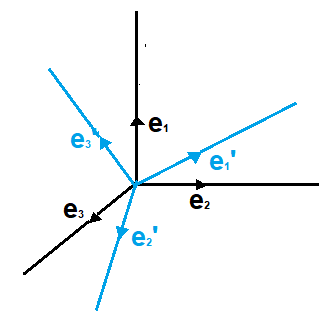
\includegraphics[width=0.3\textwidth]{figs/Rotation_of_a_coordinate_system.png}
    \caption{Example of Rotated Frames} \label{fig:rot_fme}
\end{figure}

\subsubsection{Representation} \label{sec:rotmat}
\textbf{Rotation Matrices}

We begin the study by considering only the rotation aspect of rigid body motion. 
One of the most common method to describe the orientation of coordinate frame $\mathcal{B}$ relative to
inertial frame $\mathcal{A}$ (as illustrated in Fig. \ref{fig:rot_fme}) is to sequentially rotate about the z-axis of $\mathcal{B}$ by $\alpha$, 
then y-axis of $\mathcal{B}$ by $\beta$, and finally along z-axis by $\gamma$. This yields a net rotation
of $R(\alpha, \beta, \gamma)$ and $\alpha, \gamma, \beta$ are called the ZYZ Euler angles. 

We use rotation matrix to represent a, well, rotation of coordinates. There are a number of reasons we want
to use matrices to represent such transformation:
\begin{itemize}
  \item Modern computers are highly optimized for linear algebras. \vspace{-0.5em}
  \item Rotation matrix is the cononical form for special orthogonal groups, which has proven properties
    that are useful to the representation, which we will briefly go over in section \ref{sec:so}.
\end{itemize}
\begin{equation} \label{eqn:rotmat_init}
R_{\mathbf{x}} = \begin{bmatrix}
  1 & 0 & 0\\
  0 &\cos & -\sin\\
  0 &\sin & \cos
\end{bmatrix}, 
R_{\mathbf{y}} = \begin{bmatrix}
\cos & 0 & \sin\\
0 & 1 & 0\\
-\sin & 0 & \cos
\end{bmatrix}, 
R_{\mathbf{z}} = \begin{bmatrix}
  \cos & -\sin & 0\\
  \sin & \cos & 0\\
  0 & 0 & 1
\end{bmatrix}
\end{equation}
\vspace{6pt}

A ZYZ Euler angle rotation would result in
$$ R_{ab} = R_{\mathbf{z}}(\alpha) R_{\mathbf{y}}(\beta) R_{\mathbf{z}}(\gamma) $$
We use $R_{ab}$ in the sense that it can transform coorindate points such that for point $q$ currently attached
on coordinate frame $\mathcal{A}$, and represented as $\mathbf{q}_a = [x, y ,z]$. When coordinate frame $\mathcal{B}$
rotate to frame $\mathcal{B}$, point q's relative position in the frame $\mathcal{B}$ is still $\mathbf{q}_b = [x, y, z]$, since the point
moved with the reference frame. However the current location of $\mathbf{q}_a = R_{ab} \mathbf{q}_b$

If point q rotates with frame $\mathcal{B}$ to a new frame $\mathcal{C}$, then 
$$\mathbf{q}_a = R_{ab}\mathbf{q}_b = R_{ab}R_{bc}\mathbf{q}_c$$

There exists other types of euler angle parameterizations by using different ordered sets of rotation axes,
including ZYX\footnote{roll pitch yaw} and YZX. They avoided singularity at identity orientation, however do contain
singularity at other orientations. We do not cover the details of singularity at this point, but more info at gimbal
lock\footnote{\url{https://en.wikipedia.org/wiki/Gimbal_lock}}. \vspace{1em}\\
\textbf{Quaternion}

Quaternion works in a similar way that complex number works on the unit circle to represent planar rotations. They 
give a global parameterization of $\emph{SO}(3)$ at the cost of using 4 numbers. 
$$Q = w + x\mathbf{i} + y\mathbf{j} + z\mathbf{k}$$
$w$ is the scalar component and $\mathbf{q} = (x, y, z)$ being vector component, a convenient shorthand notation being
$Q = (w, \mathbf{q})$. Vector component satisfies the following relationship
$$\mathbf{i} \cdot \mathbf{i} = \mathbf{j} \cdot \mathbf{j} = \mathbf{k} \cdot \mathbf{k} = -1$$
$$\mathbf{i} \cdot \mathbf{j} = -\mathbf{j} \cdot \mathbf{i} = \mathbf{k}, 
\mathbf{j} \cdot \mathbf{k} = -\mathbf{k} \cdot \mathbf{j} = \mathbf{i},
\mathbf{k} \cdot \mathbf{i} = -\mathbf{i} \cdot \mathbf{k} = \mathbf{j}$$

The \emph{conjugate} of a quaternion (recall imaginery numbers) $Q = (w, \mathbf{q})$ is $Q^{*} = (w, -\mathbf{q})$,
and that the magnitude of a quaternion satisfies $||Q|| = Q \cdot Q^{*}$, and the inverse of a quaternion is 
$$Q^{-1} = Q^{*} / ||Q||^{2}$$

Unit quaternions are the subset of $Q \in \mathbb{Q}$ that $||Q|| = 1$, and typically are the only type of quaternion 
we operate on. 

Similar to rotation matrices, if $Q_{ab}$, $Q_{bc}$, and $Q_{ac}$ represents rotation between frame $\mathcal{AB}$,
$\mathcal{BC}$, and $\mathcal{AC}$ respectively, the following equation holds.

$$Q_{ac} = Q_{ab} \cdot Q_{bc}$$

\subsubsection{Understanding} \label{sec:so}

\begin{figure}
  \centering
  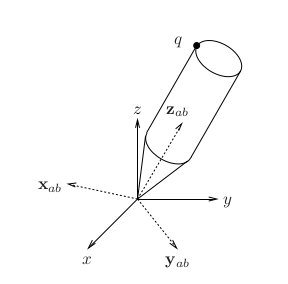
\includegraphics[width=0.5\textwidth]{figs/rot-under.png}
  \caption{Rotated Reference Frame} \label{fig:rot_showing}
\end{figure}

Consider that we have a inertial frame $\mathcal{A}$, and a body frame $\mathcal{B}$ that has undergone a rotation
about the origin point in inertial frame and no translation (Fig. \ref{fig:rot_showing}).
$\mathbf{x}_{ab}, \mathbf{y}_{ab}, \mathbf{z}_{ab}$ are
the coordinates of the principle axes of $\mathcal{B}$ in the inertial frame. Three vectors be vertical vector
and the concatenation coordinate vectors obtain
$$R_{ab} = [\mathbf{x}_{ab}, \mathbf{y}_{ab}, \mathbf{z}_{ab}]$$

Since the column vectors of $R_{ab}$ are from principle axes, dot product of the column vector with
itself is 1, otherwise 0, yielding

$$R^TR = RR^T = 1 \Rightarrow \det R = \pm 1$$

Since $\det R = \mathbf{x}^T(\mathbf{y} \times \mathbf{z})$ and that $\mathbf{x} = \mathbf{y} \times \mathbf{z}$ under
right-handed coordinate system, $\det R$ = 1. 

Therefore \textbf{right-handed coordinate frame are represented by orthogonal matrices with determinant 1}. 
The set of all matrices in $n \times n$ dimension are denoted by $\emph{SO}(n)$, as special orthogonal.
$\emph{SO}(3) \in \mathbb{R}^{3\times 3}$ is a \textbf{group} under matrix multiplication. A set $G$, with a binary
operation $\circ$ defined on elements of $G$ is considered a group if it satisfies the following axioms:
\begin{itemize}
  \setlength\itemsep{0pt}
  \item Closure: $g_1 \circ g_2 \in G$ if $g_1, g_2 \in G$
  \item Identity: exists $e$ for every $g \in G$ that $g\circ e = e\circ g = g$
  \item Inverse: for each $g \in G$ there exists a unique inverse, $g^{-1} \in G$ that $g \circ g^{-1} = g^{-1} \circ g = e$
  \item Associativity. 
\end{itemize}

In the case of $\emph{SO}(3)$, it satiefies the above criteria in that
\begin{itemize}
  \setlength\itemsep{0pt}
  \item $AB=C$ where $A, B \in \mathbb{R}^3$ gives $C\in \mathbb{R}^3$ by definition.
  \item $IR = RI = R$.
  \item $R^TR = RR^T = I$.
  \item Associativity from matrix multiplication.
\end{itemize}

\begin{figure}
  \centering
  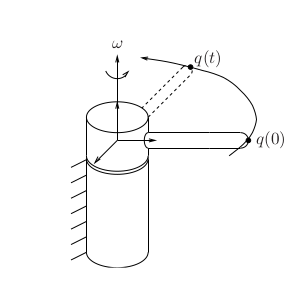
\includegraphics[width=0.5\textwidth]{figs/expo-v.png}
  \caption{Showing rotation with exponential of $\xi$} \label{fig:rot-xi}
\end{figure}

Consider the scenario in Fig. \ref{fig:rot-xi} that $\mathbf{\omega} \in \mathbb{R}^{3}$ be a unit vector specifying direction of rotation
(rotation axis) and $\theta\in \mathbb{R}$ be the angle of rotation (Rad). The velocity of the point can be written as
\begin{equation*}
  \begin{split}
    \dot{q}(t) = \omega \times q(t) = & \widehat{w}q(t)\\
    w = [w_1, w_2, w_3] \Rightarrow \widehat{w} = & \begin{bmatrix}
      0 & -w_3 & w_2 \\ w_3 & 0 & -w_1 \\ -w_2 & w_1 & 0
    \end{bmatrix}
  \end{split}
\end{equation*}
$\widehat{\omega}$ is a conversion for cross product to be represented as a typical matrix multiplication, and the equation
is a time-invariant linear differential that can be integrated to:
\begin{equation}
  \begin{split}
    q(t) = e^{\widehat{\omega}t}q(0) \\
    \therefore R(\omega, \theta) = e^{\widehat{\omega}\theta}
  \end{split}
\end{equation}
$R{\omega, \theta}$ denotes rotation about axis $\omega$ at unit velocity for $\omega$ units of time. Expand $e^{\widehat{\omega}\theta}$
using taylor expansion: 

\begin{equation} \label{eqn:tyex}
  e^{\widehat{\omega}\theta} = I + \widehat{\omega}\theta + \frac{(\widehat{\omega}\theta)^2}{2!} + \frac{(\widehat{\omega}\theta)^3}{3!} + ... 
\end{equation}

Since $\widehat{\omega}$ are skew-symmetric matrices, denote such matrices for $\mathbb{R}^3$ as $so(3), \forall S \in so(3): S^{T} = -S$. 
Through this property, $\forall \widehat{a} \in so(3)$:
\begin{equation*}
  \begin{split}
    \widehat{a}^2 = aa^T - ||a||^2I\\
    \widehat{a}^3 = -||a||^2\widehat{a}
  \end{split}
\end{equation*}
Apply the above to equation \ref{eqn:tyex}:
\begin{equation*}
  e^{\widehat{\omega}\theta} = I + \left(\theta - \frac{\theta^3}{3!} + \frac{\theta^5}{5!} - ...\right)\widehat{\omega} +
    \left(\frac{\theta^2}{2!} - \frac{\omega^4}{4!} + \frac{\omega^6}{6!} - ... \right)\widehat{\omega}^2
\end{equation*}
and hence
\begin{equation}
  \boxed{e^{\widehat{\omega}\theta} = I + \widehat{\omega}\sin\theta + \widehat{\omega}^2\left(1 - \cos\theta\right)}
\end{equation}
Commonly known as \emph{Rodrigue's formula}, we may relate this back to the rotation matrix in equation \ref{eqn:rotmat_init} of section \ref{sec:rotmat} that
\begin{equation}
  R_{\mathbf{x}}(\theta) = e^{\widehat{\mathbf{x}}\theta} = I + \left(
    \begin{bmatrix}
    0&0&0\\0&0&-1\\0&1&0
  \end{bmatrix} \sin\theta +
  \begin{bmatrix}
    0&0&0\\0&-1&0\\0&0&-1
  \end{bmatrix} (1-\cos\theta)
  \right) = \begin{bmatrix}
    1 & 0 & 0\\
    0 &\cos & -\sin\\
    0 &\sin & \cos
  \end{bmatrix}
\end{equation}
This similarly holds for rotation along other axis.

\subsection{Rigid Motion in $\mathbb{R}^3$}

\subsubsection{Representation}
As a screw motion requires a rotation and a translation component, we denote the pair of 
$(p_{ab}, R_{ab})$ as $SE(3)$ (special euclidean group) that $p\in \mathbb{R}^3, R\in SO(3)$.
Similar to the case of rotation, for $q_a, q_b$ be coordinate of $q$ in frame 
A and B, 
\begin{equation} \label{eqn:qtrans}
  {q}_a = p_{ab} + R_{ab}q_b
\end{equation}
We represent transformation in equation \ref{eqn:qtrans} in its homogenous form that
\begin{equation}
  g = \begin{bmatrix}
    R & p \\ 0 & 1
  \end{bmatrix}
\end{equation}
and if we append 1 to the coordinate of a point to yield the \emph{homogeneous coordinates}
\begin{equation}
  \bar{q} = \begin{bmatrix}
    q_1\\q_2\\q_3\\1
  \end{bmatrix}
\end{equation}
\begin{equation}
  \bar{q}_a = \begin{bmatrix} q_a\\1 \end{bmatrix}
   = \begin{bmatrix}
    p_{ab} + R_{ab}q_b\\
    1
   \end{bmatrix}
   = \begin{bmatrix} R_{ab} & p_{ab}\\0&1 \end{bmatrix}
  \begin{bmatrix}
    q_b \\ 1
  \end{bmatrix} = g_{ab}\bar{q}_b
\end{equation}
Similar to rotation components, given $g_{ab}, g_{ac}$, $g_{ac}$ can be given by the following equation
\begin{equation}
  g_{ac} = g_{ab} g_{bc} = \begin{bmatrix}
    R_{ab}R_{bc} & R_{ab}p_{bc} + p_{ab}\\0 & 1
  \end{bmatrix}
\end{equation}
This relationship can be expanded to additional reference frames. 

\subsubsection{Understanding}
We will first show that the set of rigid transformation is a group, and then link 
rigid motions and twists through exponential coordinates. 

Similar to $SO$ groups, this representation satisfies the following conditions:
\begin{itemize}
  \setlength\itemsep{0pt}
  \item If $g_1, g_2 \in SE(3)$, then $g_1g_2 \in SE(3)$
  \item The $4\times 4$ identity matrix is a member of $SE(3)$
  \item For $\bar{g} \in SE(3)$, the inverse of $\bar{g}$ is simply its matrix inversion
    \begin{equation*}
      \bar{g}^{-1} = \begin{bmatrix}
        R^{T} & -R^Tp\\0 & 1
      \end{bmatrix} = 
        \begin{bmatrix}
          R & p \\ 0 & 1
        \end{bmatrix}^{-1}
    \end{equation*}
  \item The composition rule is associative.
\end{itemize}
It is therefore a group.

Consider the scenario with the following joint that is translating and
rotating at the same time, the velocity at the tip would be
\begin{equation*}
    \dot{p}(t) = \omega \times (p(t) - q)
\end{equation*}
we can rewrite this as
\begin{equation*}
  \begin{bmatrix}
    \dot{p} \\ 0
  \end{bmatrix} = 
  \begin{bmatrix}
    \widehat{\omega} & -\omega \times q \\ 0 & 0
  \end{bmatrix}
  \begin{bmatrix}
    p \\ 1  
  \end{bmatrix} = 
  \begin{bmatrix}
    \widehat{\omega} & v \\ 0 & 0
  \end{bmatrix}
  \begin{bmatrix}
    p \\ 1  
  \end{bmatrix} = 
\end{equation*}
If we define $\xi$ as body velocity, then
\begin{equation*}
  \widehat{\xi} = \begin{bmatrix}
    \widehat{\omega} & v \\ 0 & 0
  \end{bmatrix}
\end{equation*}
therefore $\dot{p} = \widehat{\xi} p$ and differential equation solves to
\begin{equation*}
  p(t) = e^{\widehat{\xi}t}p(0)
\end{equation*}
which we may proceed similarly through taylor expansion as we did for $SO(3)$

\subsection{Velocity of a Rigid Body}
We will primarily show the process of calculating and transforming, 
velocity of particles in $SE(3)$ through the use of Twists in this section.

We will start from the rotation only situation. Consider point $q$ is fixed in
frame $B$ that is rotating along the origin of frame $A$:
\begin{equation*}
  q_A = R(t)q_B
\end{equation*}
We may describe the velocity as following
\begin{equation*}
  \begin{split}
    v_{q_a} = \omega^{s}_{ab}(t) \times q_a\\
    v_{q_b} = \omega^{b}_{ab}(t) \times q_b
  \end{split}
\end{equation*}
Where $\omega^{s}, \omega^{b}$ represents the spatial and body velocity between
frame A and B, where we may obtain them as follows.
\begin{equation*}
  \begin{split}
    \widehat{\omega}^{s}_{ab} = \dot{R}_{ab}R^{-1}_{ab}\\
    \widehat{\omega}^{b}_{ab} = R^{-1}_{ab}\dot{R}_{ab}
  \end{split}
\end{equation*}
Now we consider the general case where the motion is defined by a rigid body
transformation $g(t) \in SE(3)$. 
\begin{equation*}
  \begin{split}
    \widehat{V}^s_{ab} = \dot{g}_{ab}g^{-1}_{ab}\\
    \widehat{V}^b_{ab} = g^{-1}_{ab}\dot{g}_{ab}
  \end{split}
\end{equation*}
By doing the vee (unhat) operation, we may get the individual components of
spatial velocity
\begin{equation*}
  V^s_{ab} = \begin{bmatrix}
    v^s_{ab}\\\omega^s_{ab}
  \end{bmatrix}
\end{equation*}
And we may get the velocity of point q in frame A and B by
\begin{equation*}
  \begin{split}
    v_{q_a} = \widehat{V}^s_{ab}q_a\\
    v_{q_b} = \widehat{V}^b_{ab}q_b
  \end{split}
\end{equation*}
Further note that since both $V^{s}_{ab}$ and $V^{b}_{ab}$ are twists, 
they are related by the following relationship
\begin{equation*}
  \widehat{V}^s_{ab} = \dot{g}_{ab}g^{-1}_{ab} = g_{ab}g^{-1}_{ab}\dot{g}_{ab}g^{-1}_{ab} = g_{ab}\widehat{V}^{b}_{ab}g^{-1}_{ab}
\end{equation*}
Alternatively, 
\begin{equation*}
  V^{s}_{ab} = \begin{bmatrix}
    v^{s}_{ab}\\\omega^{s}_{ab}
  \end{bmatrix} = 
  \begin{bmatrix}
    R_{ab} & \widehat{p}_{ab}R_{ab}\\
    0 & R_{ab}
  \end{bmatrix}
  \left.\begin{bmatrix}
    v^{b}_{ab}\\\omega^b_{ab}
  \end{bmatrix}\right\}\rightarrow V^{b}_{ab}
\end{equation*}
The transformation that transforms twists from one coordiante frame to another is called
\emph{Adjoint transformation}, for one associated with $g$, denote $Ad_g$.
By one of the following methods
\begin{equation*}
  \begin{split}
    \widehat{\xi}^s & = g_{ab}\widehat{\xi}^bg^{-1}_{ab}\\
    \xi^s & = \begin{bmatrix}
      R & \widehat{p}R \\ 0 & R
    \end{bmatrix} \xi^b
  \end{split}
\end{equation*}
$Ad_g$ is invertible, and is given by the following
\begin{equation*}
  Ad_{g^{-1}} = \begin{bmatrix}
    R^T & -R^T\widehat{p} \\ 0 & R^T
  \end{bmatrix}
\end{equation*}
Knowing the velocity sets us up for planning manipulators later in the section. 

\subsection{Application}
Use the MATLAB scripts to confirm you understanding of the above material. \texttt{coordinate\_frame.m}
is intended for understanding of SO2 and SE2 groups, and \texttt{velocity\_spatial\_body.m} is for the
section on body and spatial velocity. 

\section{Manipulator Kinematics}
In this section we will briefly talks about how to utilize the knowledge in
Section \ref{sec:rbm} to simulate a manipulator. There are typically six types of
manipulator joints:
\begin{itemize}
  \setlength\itemsep{0pt}
  \item Revolute: pure rotation along a single axis
  \item Prismatic: pure linear motion along a single axis
  \item Helical: allows linear and rotation motion that are fixed to each other along the same single axis\footnote{\url{https://www.youtube.com/watch?v=fZqJopEL-k0}}. 
  \item Cylindrical: allows independent linear and rotation motion along the same single axis
  \item Spherical: allows arbitrary rotation, also refered to as \emph{ball and socket} joints
  \item Planar: allows for arbitrary translation and rotation in the plane. This is rarely used and they are typically constructed
    from a revolute joint attached to two independent prismatic joints. 
\end{itemize}
Modern manipulators are typically formulated by connecting different joints together
using rigid links. The core of the formulation is the \textbf{product of exponential}
formula, which represents the kinematics as the product of exponential of twists. 

This approach works uniformly regardless of the type of the joints and provides a global and
geometric representation of the kinematics of a manipulator which greatly simplfies
the analysis and parameterization process of a manipulator. Compared to its alternative,
\emph{Denavit–Hartenberg parameters}, it further has the advantage of only needing to
define two reference frame and easier geometric intepretation of screw axis at each joint. 

\subsection{Forward Kinematics}
The forward kinematics of a manipulator determines the configuration of the end effector
given the parameters of each joint in the manipulator. We attach
two frames, the base frame $S$\footnote{Not using $B$ to avoid confusion with body frame} and
tool frame $T$. Given a set of angles $\theta \in Q$, the forward kinematics
is a mapping $g_{st}:= Q \rightarrow SE(3)$

Typically, to compute the configuration of the end-effector, we concatenate the
rigid motion between frames.
In the example below, the transformation can be represented as 
\begin{equation} \label{eqn:fk}
  g_{s,t}(\theta_1, \theta_2) = g_{s, l_1}\left(\theta_1\right)g_{l_1, l_2}(\theta_2)g_{l_2, T}
\end{equation}

This can be extended to arbitrary number of joints on any manipulator and is a 
general formula for forward kinematics. 

\iffalse

\paragraph{A more generalized approach - questionable is we need this atm}
Equation \ref{eqn:fk} seems to rely on moving joint $\theta_2$ first and then $\theta_1$.
Using product of exponential formula we can prove that this is not the case.\textbf{Not Finished}
\begin{equation*}
  g_{st}(\theta_1, \theta_2) = e^{\widehat{\xi}_1\theta_1} e^{\widehat{\xi}_2\theta_2} g_{st}(0)
\end{equation*}

\paragraph{Manipulator Workspace}
reachable space

\fi

\subsection{Inverse Kinematics}
\subsubsection{Example IK Problem}
Inverse kinematics looks at obtaining a feasible set of parameters for joints
given a end-effector configuration. This is important since very often we receive
manipulator problems with only start and goal configurations of the end effector.
Inverse kinematics bridges the gap between the goal and our actuator. 
However note that inverse kinematics is a hard problem and general solution to
inverse kinematics, especially given high number of joints and high DoF manipulators
are active area of research and typically you won't be implementing one for yourself.

\begin{figure}
  \centering
  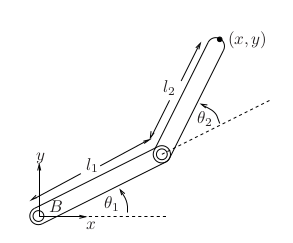
\includegraphics[width=0.4\textwidth]{figs/ik-1.png}
  \caption{Example Revolute-Revolue Manipulator} \label{fig:rrik-1}
\end{figure}

We here provide a simple 2D example of inverse kinematics of a RR manipulator (two revolute joints)
in Fig \ref{fig:rrik-1}.
The end effector locaiton can be obtained by:
\begin{equation*}
  \begin{split}
    x & = l_1\cos\theta_1 + l_2\cos(\theta_1 + \theta_2)\\
    y & = l_1\sin\theta_1 + l_2\sin(\theta_1 + \theta_2)
  \end{split}
\end{equation*}
The inverse problem would be to given $x$, and $y$ to solve for $\theta$s. 
Typically we approach the problem using polar coordinates and angles (see Fig \ref{fig:rrik-2}), because
trignometry. From the configuration visualized in above, we obtain $\theta_2$ as following
\begin{equation*}
  \theta_2 = \pi \pm \alpha, \alpha = \cos^{-1}\left(\frac{l_1^2+l_2^2-r^2}{2l_1l_2}\right)
\end{equation*}

\begin{figure}
  \centering
  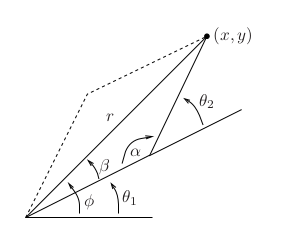
\includegraphics[width=0.4\textwidth]{figs/ik-2.png}
  \caption{RR Manipulator in Polar Coordinates} \label{fig:rrik-2}
\end{figure}

If $\alpha \neq 0$, then there are two configurations of the manipulator that would give the radius.
The second is referreed to as the "flip solution". The value of $\theta_1$ need to be solved
for each possible value for $\theta_2$, giving
\begin{equation*}
  \theta_1 = \arctan2(y,x) \pm \beta, \beta = \cos^{-1}\left(\frac{r^2+l_1^2-l_2^2}{2l_1r}\right)
\end{equation*}
This example illustrates several important aspect of IK (inverse kinematics) problems.
\begin{enumerate}
  \item One usually first divide the problem into specific subproblems. 
  \item Multiple solution occur when the desired configuration is within the workspace that
  maps to the same end-effector location. 
\end{enumerate}

There are typically two families of approach, closed-form and numeric solutions. 
Closed-form solutions are fast, analytical, and efficient calculators while numeric
requires a back-and-forth process in determine the best solution configuration. 
Yet at the heart of both, they looks at the same set of equations that defines the 
inverse kinematics problem and solve them using geometric and algebraic identities. 

\subsubsection{Application}
Use MATLAB scripts to confirm your understanding. \texttt{ik\_rr.m} is an application
of the above material. 

\iffalse
\subsubsection{Divide into subproblems}
We here briefly introduce the \emph{Paden-Kahn} subporblems, a technique
to solve inverse kinematics problem. To solve the IK problem, the method first solve 
a number of subproblems which occur frequently in inverse solutions for common maninpulato
designs, then seek to reduce the full inverse kinematics problem into subproblems
whose solutions are known. 
\fi

\subsection{Planning Manipulator Trajectory}
We are near the end of this guide and we now consider the proper planning of manipulator
via joint configuration given a end-effector trajectory.

\subsubsection{Spline Trajectory}
Spline trajectory fits the manipulator by considering the pose and twist of start
and end location. A common approach to this technique involves fitting the value of manipulator
along the curve of a spline and its first and second order derivatives trajectories. We will not be covering
this and would instead focus on the Jacobian methods as Jacobians takes an important role in robotics in
general. 

\subsubsection{Manipulator Jacobian}
Manipulators often make use of the relationship between the joint and end-effector
velocities. This has the significance that once we know desired path of the 
end-effector, we may obtain a differential of joint angles to be added onto
initial joint configuration and therefore an actionable path for the manipulator.

\begin{equation*}
  V^{s}_{st} = J^{s}_{st}(\theta)\dot{\theta}
\end{equation*}
where,
\begin{equation*}
  J^s_{st}(\theta) = \begin{bmatrix}
    \left(\frac{\partial g_{st}}{\partial \theta_1}\right)^\vee & \dots
    \left(\frac{\partial g_{st}}{\partial \theta_n}\right)^\vee
  \end{bmatrix}
\end{equation*}
$J^s_{st}$ is called a spatial manipulator jacobian that at each configuration $\theta$
it maps the joint velocity vector into the corresponding velocity of the
end-effector. Jacobian in general shows the relationship between two variables in how
the change of one affect the other.

This relationship between joint velocity and end-effector velocity can be used
to move end-effector from one configuration to another, without calculating the
inverse kinematics for the manipulator at all configuration. If $J_{st}$ is invertible,
then
\begin{equation*}
  \dot{\theta}(t) = \left(J^{s}_{st}(\theta)\right)^{-1}V^{s}_{st}(t)
\end{equation*}
And we would be able to do integration over $\theta$ to obtain a trajectory for 
$\theta$ given a known current end-effector location $g_{st}$ and known
current joint configuration $\theta$

\subsubsection{Application}
Use MATLAB scripts to confirm your understanding. Use \texttt{jacobian\_planning.m}
to perform a simple planning of manipulator. \texttt{theta\_dot.m} is required for performing integration
and you would need to fill that out as well.

\end{document}